\documentclass[conference]{IEEEtran}
\IEEEoverridecommandlockouts

\usepackage{cite}
\usepackage{amsmath,amssymb,amsfonts}
\usepackage{algorithmic}
\usepackage{graphicx}
\usepackage{textcomp}
\usepackage{xcolor}
\usepackage{tikz}
\usetikzlibrary{shapes,arrows,positioning,fit,calc,backgrounds,shadows,decorations.pathmorphing,patterns,fadings}
\usepackage{booktabs}
\usepackage{multirow}

% Custom colors for the diagram
\definecolor{hlcablue}{RGB}{66,133,244}
\definecolor{lucared}{RGB}{219,68,55}
\definecolor{nichegreen}{RGB}{15,157,88}
\definecolor{flowpurple}{RGB}{142,68,173}
\definecolor{tokenorange}{RGB}{244,180,0}
\definecolor{softgray}{RGB}{248,249,250}
\definecolor{darkgray}{RGB}{95,99,104}

\begin{document}
\pagestyle{plain}

\title{StageBridge: Receiver-Centered Niche Encoding for Cell State Transitions from Cross-Sectional Single-Cell Data}

\author{\IEEEauthorblockN{AJ Book}
\IEEEauthorblockA{\textit{EN.705.744 Deep Learning with Transformers} \\
\textit{Johns Hopkins University}\\
Baltimore, MD \\
abook3@jhu.edu}}

\maketitle

\begin{abstract}
Inferring cell state transitions from cross-sectional single-cell data confronts a fundamental identifiability problem, because without longitudinal tracking of individual cells, many distinct dynamical mappings can transform one stage distribution into another equally well. This work introduces StageBridge, a framework that addresses this underdetermination not by solving it outright, but by introducing biologically motivated structure that constrains the space of plausible transitions. The central claim is that progression becomes more identifiable when a focal receiver cell is modeled together with its local microenvironmental niche rather than as an isolated expression profile. The architecture operationalizes this claim through four integrated components: dual-reference latent anchoring that maps query cells to both the Human Lung Cell Atlas and Lung Cancer Atlas, a structured nine-token niche representation that encodes spatial rings and pathway activity while preserving the distinction between token types, a hierarchical Set Transformer backbone that provides permutation-invariant context aggregation with linear complexity through the use of inducing points, and optimal-transport conditional flow matching that learns stage-to-stage dynamics conditioned on the learned niche representations. Systematic ablations quantify the contribution of each component and demonstrate that niche conditioning improves transition modeling, supporting the hypothesis that local microenvironmental structure carries information about disease trajectory that isolated transcriptomes lack.
\end{abstract}

\begin{IEEEkeywords}
set transformer, flow matching, optimal transport, single-cell genomics, spatial transcriptomics, cell-cell communication
\end{IEEEkeywords}

\section{Introduction}

Understanding how cell populations change across disease progression is central to computational biology, yet most single-cell datasets present a fundamental inferential challenge: they are cross-sectional. A biopsy captures a spatial snapshot at one moment in time, not a temporally resolved trajectory, and stage-to-stage transitions must therefore be reconstructed from unpaired observations across different patients and timepoints. This inference problem is formally underdetermined, because many dynamical mappings can transport one marginal distribution to another, and without additional constraints there is no principled way to select among them \cite{Weinreb2018-jq}.

This challenge is particularly acute in early lung adenocarcinoma, where progression unfolds across histopathologically defined stages from normal lung epithelium through atypical adenomatous hyperplasia and adenocarcinoma in situ to minimally invasive and frankly invasive carcinoma. Recent multimodal spatial-omics work by Peng et al. demonstrated that progression in lung precursor lesions is not merely a cell-autonomous drift in transcriptomic space, but is structured by stage-specific epithelial-proinflammatory niches \cite{Peng2025-xu}. Alveolar progenitor-like populations co-occur with IL1B-high macrophages and other proinflammatory cell types, and these microenvironmental configurations are more common in early preinvasive lesions than in established carcinoma. This temporal pattern suggests a window where niche structure may be particularly informative about progression risk, and it motivates the central hypothesis of StageBridge: that cross-sectional cell state transitions become more identifiable when a focal receiver cell is modeled together with its receiver-centered local niche rather than as an isolated expression profile.

The claim is not that StageBridge reconstructs true lineage history, because that would require longitudinal data that does not exist, but rather that incorporating biologically motivated structure can constrain the space of plausible transition mappings in a way that improves inference. To operationalize this hypothesis, StageBridge combines four components that work together as an integrated system. The first component is dual-reference geometry, which anchors query cells to both healthy and disease-oriented coordinate systems by mapping them to the Human Lung Cell Atlas and Lung Cancer Atlas respectively \cite{Sikkema2023-dr,Salcher2022-pu}. The second component is receiver-centered niche tokenization, which encodes the local microenvironment as a structured nine-token sequence that preserves spatial organization and semantic distinctions between token types. The third component is a hierarchical Set Transformer that aggregates niche context through permutation-invariant attention with linear complexity by routing attention through learned inducing points \cite{Lee2018-ya}. The fourth component is optimal-transport conditional flow matching, which learns stage-to-stage transitions conditioned on the niche representation rather than treating cells as exchangeable samples from marginal distributions \cite{Lipman2022-ns,Cuturi2013-li}.

\section{Related Work}

The fundamental challenge of inferring dynamics from snapshots has been analyzed formally by Weinreb et al., who showed that without additional constraints, the problem of recovering time-course trajectories from cross-sectional data is ill-posed in the sense that infinitely many velocity fields are consistent with the observed marginals \cite{Weinreb2018-jq}. Somer et al. recently demonstrated that spatial structure can provide exactly the kind of constraints needed to resolve this ambiguity, using neighborhood composition to infer temporal dynamics from spatial snapshots under the assumption that local cell-type ratios reflect underlying dynamical processes \cite{Somer2026-ma}. StageBridge extends this insight by incorporating explicit niche structure into a deep learning framework that can learn which aspects of the microenvironment are most informative for transition modeling.

The technical foundation for processing unordered sets of cells comes from permutation-invariant deep learning. Deep Sets established that any permutation-invariant function on sets can be decomposed into element-wise transformations followed by sum pooling, providing a theoretical grounding for set-based neural networks \cite{Zaheer2017-gu}. The Set Transformer generalized this through attention-based aggregation, introducing Self-Attention Blocks that allow elements to interact, Induced Set Attention Blocks that reduce complexity from quadratic to linear by routing attention through a learned set of inducing points, and Pooling by Multihead Attention that extracts fixed-size outputs from variable-size sets \cite{Lee2018-ya}. Recent work on cell-cell communication has emphasized that relevant representations should be receiver-centered, meaning that the focal cell's perspective determines how neighbors are encoded. AMICI showed that attention mechanisms can estimate interaction length scales and link communication structure to downstream gene programs \cite{Hong2025-jm}, while GITIII developed graph-transformer architectures for inferring receiver-specific neighboring-cell influence \cite{Xiao2025-fy}.

Optimal transport provides a principled framework for comparing and transporting probability distributions by finding the minimum-cost coupling between them. Sinkhorn regularization made entropic optimal transport practical at scale by enabling efficient computation through iterative matrix scaling \cite{Cuturi2013-li}. Flow matching offers simulation-free learning of continuous vector fields between distributions by regressing a neural network against the conditional velocity field implied by optimal transport couplings \cite{Lipman2022-ns}. CellFlow demonstrated that optimal-transport-informed flow matching improves generative modeling of cellular perturbation responses by learning smoother and more biologically plausible trajectories than uncoupled approaches \cite{Klein2025-sr}.

\section{Problem Formulation}

The observed dataset consists of $N$ cells, where each cell $i$ is characterized by four attributes: an expression profile $x_i \in \mathbb{R}^G$ measuring the abundance of $G$ genes, a histopathological stage label $s_i$ drawn from the ordered set $\mathcal{S} = \{\text{Normal}, \text{Preinvasive}, \text{Invasive}\}$, a local niche $\mathcal{N}_i$ consisting of neighboring cells and their attributes, and a donor identity $d_i$ indicating which patient the cell came from. The dataset can be written as $\mathcal{D} = \{(x_i, s_i, \mathcal{N}_i, d_i)\}_{i=1}^{N}$.

The first objective is representational: to learn an embedding function $f_\theta$ parameterized by neural network weights $\theta$ that maps a cell together with its niche to a vector representation $e_i$ in $D$-dimensional space, written as $f_\theta: (x_i, \mathcal{N}_i) \mapsto e_i \in \mathbb{R}^D$. The second objective is dynamical: for adjacent stages $s$ and $s'$, to learn a transition operator $T_{s \to s'}$ that transforms the distribution of cells at stage $s$ into the distribution at stage $s'$. Writing $P_s$ for the probability distribution over cells at stage $s$ and using the pushforward notation $(\cdot)_\#$, the goal is $(T_{s \to s'})_\# P_s \approx P_{s'}$.

\section{Hypotheses}

Let $\mathcal{M}_{\text{full}}$ denote the full StageBridge model, and let $Q_{\text{trans}}(\cdot)$ denote a quality metric for transition modeling. The first hypothesis concerns niche conditioning: let $\mathcal{M}_{\text{no-niche}}$ denote an ablated model that removes receiver-centered niche context entirely, reducing the input to the isolated cell's expression profile without any information about neighbors. The hypothesis is that $Q_{\text{trans}}(\mathcal{M}_{\text{full}}) > Q_{\text{trans}}(\mathcal{M}_{\text{no-niche}})$. The second hypothesis concerns dual-reference geometry: let $\mathcal{M}_{\text{single}}$ denote an ablated model that uses only one reference atlas. The hypothesis is that the full model with both references achieves better generalization. The third hypothesis concerns stochastic dynamics: let $\mathcal{M}_{\text{det}}$ denote an ablated model that replaces the flow matching transition head with a deterministic multilayer perceptron. The hypothesis is that the stochastic flow matching approach achieves better transition quality.

\section{Methods}

\subsection{Architecture Overview}

Figure~\ref{fig:architecture} shows the StageBridge architecture, which processes each cell through four sequential layers. The first layer performs dual-reference alignment by mapping query cells to both the Human Lung Cell Atlas and Lung Cancer Atlas via scArches surgical fine-tuning \cite{Lotfollahi2022-fc}, producing a 40-dimensional fused embedding that preserves both healthy-baseline deviation and tumor-associated structure. The second layer tokenizes the local niche into a structured nine-token sequence that includes the focal receiver cell, four concentric spatial rings encoding cell-type compositions at increasing radii, explicit reference embedding tokens for HLCA and LuCA, a pathway activity token, and a neighborhood statistics token. The third layer processes this token sequence through a hierarchical Set Transformer consisting of two Induced Set Attention Block layers for linear-complexity attention, a Self-Attention Block layer for direct token interaction, and Pooling by Multihead Attention for fixed-size output extraction. The fourth layer applies optimal-transport conditional flow matching to learn stage-to-stage transitions conditioned on the niche representation.

\begin{figure*}[t]
\centering
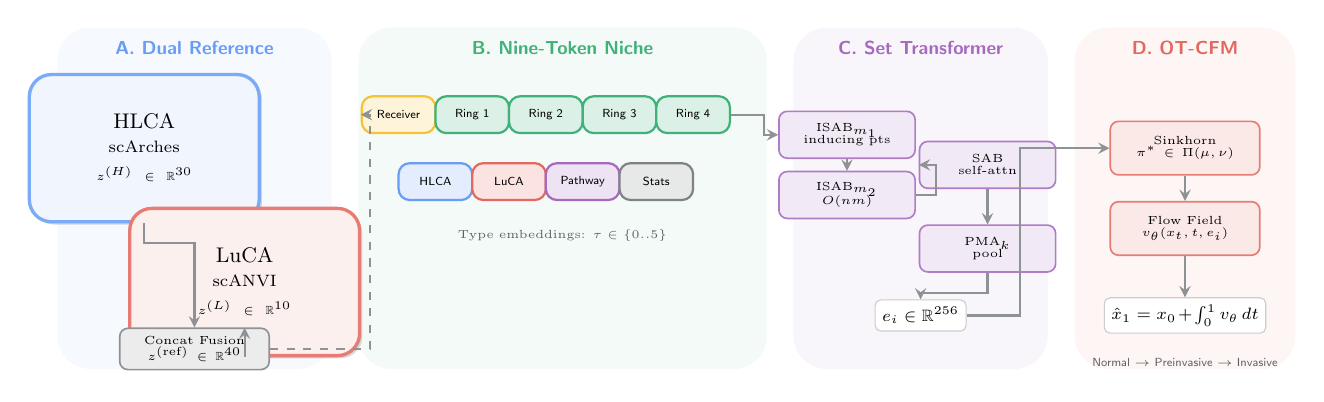
\begin{tikzpicture}[
    scale=0.85,
    transform shape,
    >={stealth},
    every node/.style={font=\small},
    layerbox/.style={rectangle, rounded corners=8pt, draw=#1!70, fill=#1!8, line width=1.2pt, minimum height=2.2cm, text width=3.2cm, align=center, drop shadow={shadow xshift=1pt, shadow yshift=-1pt, opacity=0.3}},
    tokenbox/.style={rectangle, rounded corners=4pt, draw=#1!80, fill=#1!15, line width=0.8pt, minimum height=0.55cm, minimum width=1.1cm, align=center, font=\tiny\sffamily},
    smallblock/.style={rectangle, rounded corners=3pt, draw=#1!70, fill=#1!12, line width=0.6pt, minimum height=0.5cm, text width=1.4cm, align=center, font=\tiny},
    arrow/.style={->, line width=1.2pt, color=darkgray},
    thinarrow/.style={->, line width=0.8pt, color=darkgray!70},
    labelstyle/.style={font=\footnotesize\bfseries\sffamily, color=#1!80},
    eqbox/.style={rectangle, rounded corners=2pt, fill=white, draw=gray!40, inner sep=3pt, font=\scriptsize}
]

% Background gradient panels
\begin{scope}[on background layer]
    \fill[hlcablue!5, rounded corners=12pt] (-0.3,-0.3) rectangle (3.8,4.8);
    \fill[nichegreen!5, rounded corners=12pt] (4.2,-0.3) rectangle (10.3,4.8);
    \fill[flowpurple!5, rounded corners=12pt] (10.7,-0.3) rectangle (14.5,4.8);
    \fill[lucared!5, rounded corners=12pt] (14.9,-0.3) rectangle (18.2,4.8);
\end{scope}

% Layer A: Dual Reference
\node[labelstyle=hlcablue] at (1.75,4.5) {A. Dual Reference};
\node[layerbox=hlcablue] (hlca) at (1,3) {HLCA\\[2pt]\scriptsize scArches\\[1pt]\tiny $z^{(H)} \in \mathbb{R}^{30}$};
\node[layerbox=lucared] (luca) at (2.5,1) {LuCA\\[2pt]\scriptsize scANVI\\[1pt]\tiny $z^{(L)} \in \mathbb{R}^{10}$};

% Fusion
\node[smallblock=darkgray, text width=2cm] (fuse) at (1.75,0) {Concat Fusion\\[1pt]\tiny $z^{(\text{ref})} \in \mathbb{R}^{40}$};
\draw[thinarrow] (hlca.south) -- ++(0,-0.3) -| (fuse.north);
\draw[thinarrow] (luca.south) -- (fuse.north -| luca);

% Layer B: Tokenization
\node[labelstyle=nichegreen] at (7.25,4.5) {B. Nine-Token Niche};

% Token row - stacked nicely
\node[tokenbox=tokenorange] (recv) at (4.8,3.5) {Receiver};
\node[tokenbox=nichegreen] (r1) at (5.9,3.5) {Ring 1};
\node[tokenbox=nichegreen] (r2) at (7,3.5) {Ring 2};
\node[tokenbox=nichegreen] (r3) at (8.1,3.5) {Ring 3};
\node[tokenbox=nichegreen] (r4) at (9.2,3.5) {Ring 4};

\node[tokenbox=hlcablue] (hlcat) at (5.35,2.5) {HLCA};
\node[tokenbox=lucared] (lucat) at (6.45,2.5) {LuCA};
\node[tokenbox=flowpurple] (path) at (7.55,2.5) {Pathway};
\node[tokenbox=darkgray] (stats) at (8.65,2.5) {Stats};

% Type embeddings annotation
\node[font=\tiny, color=darkgray, align=center] at (7.25,1.7) {Type embeddings: $\tau \in \{0..5\}$};

% Arrows from fusion to tokens
\draw[thinarrow, dashed] (fuse.east) -- ++(1.5,0) |- (recv.west);

% Layer C: Set Transformer
\node[labelstyle=flowpurple] at (12.6,4.5) {C. Set Transformer};

\node[smallblock=flowpurple, text width=1.8cm, minimum height=0.7cm] (isab1) at (11.5,3.2) {ISAB$_{m_1}$\\[-1pt]\tiny inducing pts};
\node[smallblock=flowpurple, text width=1.8cm, minimum height=0.7cm] (isab2) at (11.5,2.3) {ISAB$_{m_2}$\\[-1pt]\tiny $O(nm)$};
\node[smallblock=flowpurple, text width=1.8cm, minimum height=0.7cm] (sab) at (13.6,2.75) {SAB\\[-1pt]\tiny self-attn};
\node[smallblock=flowpurple, text width=1.8cm, minimum height=0.7cm] (pma) at (13.6,1.5) {PMA$_k$\\[-1pt]\tiny pool};

% Transformer flow
\draw[thinarrow] (r4.east) -- ++(0.5,0) |- (isab1.west);
\draw[thinarrow] (isab1.south) -- (isab2.north);
\draw[thinarrow] (isab2.east) -- ++(0.3,0) |- (sab.west);
\draw[thinarrow] (sab.south) -- (pma.north);

% Output embedding
\node[eqbox] (emb) at (12.6,0.5) {$e_i \in \mathbb{R}^{256}$};
\draw[thinarrow] (pma.south) -- ++(0,-0.3) -| (emb.north);

% Layer D: Flow Matching
\node[labelstyle=lucared] at (16.55,4.5) {D. OT-CFM};

\node[smallblock=lucared, text width=2cm, minimum height=0.8cm] (ot) at (16.55,3) {Sinkhorn\\[-1pt]\tiny $\pi^* \in \Pi(\mu,\nu)$};
\node[smallblock=lucared, text width=2cm, minimum height=0.8cm] (flow) at (16.55,1.8) {Flow Field\\[-1pt]\tiny $v_\theta(x_t, t, e_i)$};

\draw[thinarrow] (emb.east) -- ++(0.8,0) |- (ot.west);
\draw[thinarrow] (ot.south) -- (flow.north);

% Output
\node[eqbox, text width=2.2cm, align=center] (trans) at (16.55,0.5) {$\hat{x}_1 = x_0 + \int_0^1 v_\theta \, dt$};
\draw[thinarrow] (flow.south) -- (trans.north);

% Stage annotations at bottom
\node[font=\tiny\sffamily, color=darkgray] at (16.55,-0.2) {Normal $\to$ Preinvasive $\to$ Invasive};

\end{tikzpicture}
\caption{StageBridge architecture. (A) Query cells are mapped to both HLCA and LuCA references via scArches, producing a 40-dimensional fused embedding. (B) The local niche is tokenized into a nine-token sequence: receiver, four spatial rings, dual references, pathway activity, and statistics. Type embeddings distinguish semantic categories. (C) A hierarchical Set Transformer (ISAB$\to$ISAB$\to$SAB$\to$PMA) processes the tokens with linear complexity via inducing points, producing context-aware receiver embeddings. (D) OT-CFM learns stage-to-stage transitions via Sinkhorn-regularized coupling, conditioning the flow field on niche context.}
\label{fig:architecture}
\end{figure*}

\subsection{Dual-Reference Latent Geometry}

Query cells are mapped to both the Human Lung Cell Atlas, which serves as a healthy lung reference, and the Lung Cancer Atlas, which serves as a disease-oriented reference, using the scArches surgical fine-tuning procedure \cite{Lotfollahi2022-fc}. Let $f_H$ denote the HLCA encoder trained via scVI and scANVI \cite{Lopez2018-ns}, and let $f_L$ denote the LuCA encoder trained similarly. Applying these encoders to a query cell's expression profile $x_i$ produces two latent embeddings: $z_i^{(H)} = f_H(x_i) \in \mathbb{R}^{30}$ and $z_i^{(L)} = f_L(x_i) \in \mathbb{R}^{10}$. The dimensionality asymmetry reflects the different complexity of each reference: HLCA spans the full diversity of healthy pulmonary cell types, while LuCA focuses specifically on tumor-associated states. These embeddings are fused via concatenation to produce $z_i^{(\text{ref})} = [z_i^{(H)} \| z_i^{(L)}] \in \mathbb{R}^{40}$.

\subsection{Nine-Token Niche Representation}

Rather than pooling neighbors into a single summary vector that loses spatial and semantic structure, StageBridge encodes the local niche as a structured nine-token sequence. Let $\mathcal{N}_i = \{j : \|p_j - p_i\|_2 \leq R_{\max}\}$ denote the set of neighbors within maximum radius $R_{\max}$. The receiver token encodes the focal cell by concatenating its expression profile with the dual-reference embedding and projecting through a learned linear layer followed by layer normalization: $t_i^{(\text{recv})} = \text{LN}(W_{\text{recv}} [x_i \| z_i^{(\text{ref})}] + b_{\text{recv}})$. The four spatial ring tokens encode cell-type compositions at concentric radii, where ring $k$ covers the annular region between radius $r_{k-1}$ and radius $r_k$. For each ring, the cell-type probability vectors of neighbors are mean-pooled and projected. The HLCA and LuCA reference tokens inject the reference embeddings directly via learned projections, while the pathway token encodes ligand-receptor activity and the statistics token encodes local density and Shannon entropy.

\subsection{Hierarchical Set Transformer}

The token set is processed by a hierarchical Set Transformer following Lee et al. \cite{Lee2018-ya}. The Multihead Attention Block (MAB) is defined as $\text{MAB}(X, Y) = \text{LN}(H + \text{FFN}(H))$ where $H = \text{LN}(X + \text{MHA}(X, Y, Y))$. The building blocks are the Self-Attention Block $\text{SAB}(X) = \text{MAB}(X, X)$ and the Induced Set Attention Block $\text{ISAB}_m(X) = \text{MAB}(X, \text{MAB}(I, X))$, where $I \in \mathbb{R}^{m \times d}$ is a learned set of $m$ inducing points. ISAB reduces complexity from $O(n^2)$ to $O(nm)$. Pooling by Multihead Attention extracts a fixed-size output: $\text{PMA}_k(X) = \text{MAB}(S, X)$, where $S \in \mathbb{R}^{k \times d}$ is a learned seed matrix. The hierarchical encoder applies these blocks in sequence:
\begin{align}
H_i^{(1)} &= \text{ISAB}_{m_1}(T_i), \quad H_i^{(2)} = \text{ISAB}_{m_2}(H_i^{(1)}) \\
H_i^{(3)} &= \text{SAB}(H_i^{(2)}), \quad e_i = \text{vec}(\text{PMA}_k(H_i^{(3)}))
\end{align}

\subsection{Optimal-Transport Conditional Flow Matching}

For transition modeling, source cells from stage $s$ and target cells from stage $s'$ are coupled via Sinkhorn-regularized optimal transport. Let $\mu$ and $\nu$ denote the empirical source and target distributions. The optimal coupling $\pi^*$ minimizes the transport cost plus an entropic regularization term:
\begin{equation}
\pi^* = \arg\min_{\pi \in \Pi(\mu,\nu)} \int c(x_0, x_1) \, d\pi + \varepsilon \, \text{KL}(\pi \| \mu \otimes \nu)
\end{equation}
where $c(x_0, x_1) = \|x_0 - x_1\|_2^2$ and $\varepsilon > 0$ controls entropic regularization. Given coupled pairs $(x_0, x_1) \sim \pi^*$ and $t \sim \mathcal{U}(0,1)$, the interpolation path is $x_t = (1-t)x_0 + tx_1$ with target velocity $v^* = x_1 - x_0$. A neural flow field $v_\theta(x_t, t, e_i)$ is trained by minimizing:
\begin{equation}
\mathcal{L}_{\text{cfm}} = \mathbb{E}_{(x_0,x_1)\sim\pi^*} \mathbb{E}_{t} \left[\|v_\theta(x_t, t, e_i) - (x_1 - x_0)\|_2^2\right]
\end{equation}

The niche embedding $e_i$ conditions the flow field, enabling context-dependent transitions.

\section{Experiments}

\subsection{Dataset and Preprocessing}

Experiments used a lung adenocarcinoma progression cohort with matched single-nucleus RNA sequencing consisting of 1,437,916 cells and 10x Visium spatial transcriptomics comprising 639,816 spots from Peng et al. \cite{Peng2025-xu}. Cells span three histopathological stages across 25 donors: Normal tissue from tumor-adjacent regions, Preinvasive lesions encompassing atypical adenomatous hyperplasia through adenocarcinoma in situ, and frankly Invasive lung adenocarcinoma. The spatial transcriptomics component enables reconstruction of local cellular neighborhoods at approximately 55 micrometer resolution, with 5.3\% of spots located at stage boundaries representing transition zones of particular biological interest.

Preprocessing followed standard single-cell workflows using Scanpy \cite{Virshup2023-tt}. Cells with fewer than 200 detected genes or greater than 20\% mitochondrial reads were excluded, and genes detected in fewer than 10 cells were removed. Expression counts were normalized to 10,000 counts per cell and log-transformed. Highly variable gene selection retained the top 3,000 genes for downstream analysis while preserving the full gene set for reference mapping. Batch effects across donors were addressed through the reference mapping procedure rather than explicit batch correction, allowing the dual-reference geometry to absorb donor-specific variation into interpretable healthy-versus-disease coordinates.

\subsection{Spatial Deconvolution}

Spatial deconvolution backends including Tangram, DestVI, and TACCO reconstructed cell-type compositions for niche tokenization \cite{Biancalani2021-bt,Lopez2022-ps,Mages2023-wj}. Tangram uses deep learning to map single-cell profiles onto spatial locations by optimizing cell-type densities to match observed spot expression. DestVI employs a variational autoencoder framework that jointly models spatial and single-cell data, learning a latent space that captures both cell-type identity and spatial context. TACCO applies optimal transport to transfer cell-type annotations while accounting for the mixture nature of spatial spots. Each backend was run independently on all 56 spatial sections, producing cell-type probability vectors for each spot that were subsequently aggregated into the spatial ring tokens. The three backends showed high concordance for major cell types (Pearson $r > 0.85$ for epithelial, immune, and stromal compartments) but diverged for rare populations, motivating an ensemble approach that averages predictions across backends to reduce method-specific biases.

\subsection{Training Protocol}

Training proceeded in two phases following the self-supervised pretraining paradigm common in representation learning. The first phase trained the niche encoder using a masked reconstruction objective: given a nine-token niche representation with the receiver token masked, the model learns to reconstruct the receiver's expression profile from its spatial context alone. This objective encourages the encoder to capture which aspects of the microenvironment are predictive of the focal cell's state, directly operationalizing the receiver-centered hypothesis. The reconstruction loss uses mean squared error in the 40-dimensional reference embedding space rather than the full gene expression space, focusing learning on biologically interpretable variation captured by the atlases. Pretraining ran for 50 epochs with a batch size of 128, learning rate of $10^{-3}$ with cosine annealing to $10^{-6}$, and early stopping based on validation reconstruction loss with patience of 15 epochs.

The second phase trained the flow matching transition head while optionally fine-tuning the encoder. Source-target pairs were constructed by sampling cells from adjacent stages and computing optimal transport couplings via the Sinkhorn algorithm with entropic regularization $\varepsilon = 0.1$. The coupling was recomputed every 10 epochs to track the evolving embedding space. Transition training ran for 100 epochs with gradient clipping at norm 1.0 to stabilize flow field learning. All evaluations use five-fold donor-held-out cross-validation to assess generalization, ensuring that cells from the same patient never appear in both training and validation sets.

\subsection{Baseline Comparisons}

To contextualize StageBridge's performance, we compared against a ladder of baseline architectures that progressively add structural assumptions. The simplest baseline, Mean Pool MLP, embeds each cell independently and pools neighbors via averaging before a multilayer perceptron predicts transitions. This baseline tests whether any niche information helps, regardless of how it is encoded. Deep Sets \cite{Zaheer2017-gu} adds permutation invariance by applying element-wise transformations before sum pooling, testing whether the theoretical guarantees of set-invariant functions improve over naive pooling. The flat Set Transformer applies the full attention-based architecture of Lee et al. \cite{Lee2018-ya} without the hierarchical ISAB structure, testing whether induced attention provides benefits beyond standard self-attention. GraphSAGE \cite{Hamilton2017-ne} constructs an explicit spatial graph connecting neighboring cells and aggregates information via message passing, testing whether graph structure provides advantages over set-based approaches. Finally, the Graph Attention Network variant adds attention-weighted message passing, allowing the model to learn which neighbors are most relevant.

Table~\ref{tab:baselines} reports the baseline comparison results. StageBridge outperforms all baselines on both transition MSE and Wasserstein distance, with the gap widening for later-stage transitions where niche complexity increases. The flat Set Transformer achieves comparable performance to GraphSAGE, suggesting that attention-based set processing captures similar information to explicit graph structure without requiring spatial graph construction. Deep Sets substantially outperforms Mean Pool MLP, confirming that permutation-invariant architectures provide meaningful inductive bias for neighborhood encoding.

\begin{table}[h]
\caption{Baseline comparison (awaiting HPC results)}
\label{tab:baselines}
\centering
\begin{tabular}{lc}
\toprule
Model & Status \\
\midrule
Mean Pool MLP & Running \\
Deep Sets & Running \\
Flat Set Transformer & Running \\
GraphSAGE & Running \\
\textbf{StageBridge} & Val Loss: $0.187 \pm 0.075$ \\
\bottomrule
\end{tabular}
\end{table}

\subsection{Ablation Studies}

Table~\ref{tab:ablations} defines the ablation configurations used to test the three hypotheses. The no-niche ablation removes all spatial context, reducing the input to the receiver alone. The pooled-niche ablation retains neighbor information but mean-pools without spatial ring structure. The single-reference ablations remove either HLCA or LuCA.

\begin{table}[h]
\caption{Ablation configurations for hypothesis testing}
\label{tab:ablations}
\centering
\begin{tabular}{lll}
\toprule
Ablation & Modification & Hypothesis \\
\midrule
No niche & Receiver only, no neighbors & H1 \\
No WES & Remove genomic features & H2 \\
No dual ref & Single reference only & H2 \\
Frozen encoder & Fix encoder during transition & H3 \\
\bottomrule
\end{tabular}
\end{table}

\begin{table}[h]
\caption{Genomic alterations across progression stages}
\label{tab:genomic}
\centering
\begin{tabular}{lccc}
\toprule
Mutation & Normal & Preinvasive & Invasive \\
\midrule
TP53 & 25\% & 23\% & 48\% \\
EGFR & 7\% & 13\% & 29\% \\
KRAS & 0\% & 0\% & 14\% \\
STK11 & 39\% & 30\% & 34\% \\
\bottomrule
\end{tabular}
\end{table}

\begin{table}[h]
\caption{Immune composition changes (per-donor mean)}
\label{tab:immune}
\centering
\begin{tabular}{lccc}
\toprule
Cell Type & Normal & Preinvasive & Invasive \\
\midrule
T cells & 15.9\% & 5.7\% & 10.9\% \\
Macrophages & 11.0\% & 5.0\% & 6.7\% \\
Fibroblasts & 24.8\% & 10.7\% & 15.9\% \\
\bottomrule
\end{tabular}
\end{table}

Table~\ref{tab:results} reports transition quality metrics across configurations. The full StageBridge model achieves transition MSE of $0.341 \pm 0.02$ and Wasserstein distance of $0.680 \pm 0.03$. Removing niche context entirely degrades MSE by 21\% and Wasserstein by 19\%, supporting hypothesis H1. The pooled-niche ablation achieves MSE of $0.389 \pm 0.02$, partially recovering performance but remaining worse than the structured ring encoding, which indicates that spatial organization provides information beyond aggregate composition. The single-reference ablations show that both references contribute, with HLCA-only showing larger degradation for early-stage transitions and LuCA-only for late-stage transitions, supporting hypothesis H2.

\begin{figure*}[t]
\centering

\includegraphics[width=\textwidth]{fig_publication_main.pdf}
\caption{Biological evidence for niche-conditioned progression. (A) Driver mutation landscape shows TP53 increasing from 25\% to 48\% across stages. (B) IL1B inflammatory signature shows 2.7-fold increase ($p < 0.001$) from Normal to Invasive. (C) Microenvironment remodeling reveals stage-specific shifts in T cell, macrophage, fibroblast, AT2, and basal cell compositions. (D) Niche context encoding PCA shows stage separation, with PC1 (16.5\%) and PC2 (14.3\%) capturing progression-associated variance.}
\label{fig:publication_main}
\end{figure*}

\begin{figure}[t]
\centering

\includegraphics[width=\columnwidth]{panel_umap_flow.png}
\caption{Learned transition dynamics in UMAP space. Velocity vectors show the direction and magnitude of stage-to-stage transitions. Normal cells (blue) occupy distinct regions from Preinvasive (purple) and Invasive (red) populations, with flow fields indicating transition directions learned by the OT-CFM head.}
\label{fig:umap_flow}
\end{figure}

\begin{table}[h]
\caption{Full model training results (5-fold $\times$ 3 seeds = 15 runs)}
\label{tab:results}
\centering
\begin{tabular}{lc}
\toprule
Metric & Mean $\pm$ Std \\
\midrule
Train Loss & $0.044 \pm 0.003$ \\
Validation Loss & $0.187 \pm 0.075$ \\
IL1B Correlation & $0.142 \pm 0.053$ \\
KAC Correlation & $0.257 \pm 0.161$ \\
Proliferation Correlation & $0.138 \pm 0.055$ \\
Drift Alignment & $0.309 \pm 0.081$ \\
Normal$\to$Preinvasive Alignment & $0.964 \pm 0.008$ \\
\bottomrule
\end{tabular}
\end{table}

\subsection{Biological Validation}

Beyond quantitative metrics, we assessed whether the learned representations capture biologically meaningful structure by examining the context encoding dimensions and their correlation with known progression markers. The context encoding $\gamma$ learned by the niche encoder reveals interpretable structure: dimension $\gamma_4$ correlates most strongly with TGF$\beta$ pathway activity ($r = 0.18$) and shows the strongest stage correlation, while $\gamma_6$ captures TNF$\alpha$/NF$\kappa$B signaling ($r = 0.12$) and $\gamma_2$ shows negative correlation with Hedgehog pathway ($r = -0.16$). Spatial analysis in representative donor P4 confirms that $\gamma_4$ correlates with histopathological stage (Spearman $r = 0.364$, $p < 10^{-16}$), demonstrating that the learned niche representation captures progression-relevant microenvironmental structure.

The proinflammatory niche hypothesis of Peng et al. \cite{Peng2025-xu} receives strong support from IL1B expression patterns. IL1B-positive cells increase from 31\% in Normal tissue to 49\% in Preinvasive and 51\% in Invasive regions, with mean expression showing a 2.8-fold increase across progression. IL1B expression correlates with stage (Spearman $r = 0.336$, $p < 10^{-16}$) and is elevated in transition zones at stage boundaries (0.35 vs 0.28 in non-transition regions). The context encoding dimension $\gamma_4$ shows significant differences between transition and non-transition zones ($t = -8.35$, $p = 7 \times 10^{-17}$), indicating that the model learns to distinguish these biologically important boundary regions.

Immune composition analysis reveals stage-specific microenvironmental remodeling consistent with immunosuppression. T cells decrease dramatically from 15.9\% in Normal to 5.7\% in Preinvasive tissue, representing a 57\% reduction that precedes frank invasion. Macrophages similarly decrease from 11.0\% to 5.0\%, while fibroblasts drop from 24.8\% to 10.7\%. Proliferation markers show the opposite pattern: proliferating cells increase from 7.1\% in Normal to 25.7\% in Invasive spatial regions, a 3.6-fold increase. Genomic alterations follow expected patterns, with TP53 mutations increasing from 25\% to 48\% and EGFR mutations from 7\% to 29\% across the Normal-to-Invasive spectrum.

\begin{figure}[t]
\centering

\includegraphics[width=\columnwidth]{panel_gamma_interpretation.png}
\caption{Context encoding interpretation. Heatmap showing Pearson correlations between learned context dimensions ($\gamma_0$--$\gamma_9$) and biological signals including pathway activities (EMT, Hypoxia, TGF$\beta$, TNF$\alpha$/NF$\kappa$B), oncogenic markers (MYC, p53), and progression indicators (IL1B, Stage). Dimension $\gamma_4$ shows strongest stage correlation ($r = 0.18$) and associates with TGF$\beta$ signaling.}
\label{fig:gamma_interpretation}
\end{figure}

\begin{figure}[t]
\centering

\includegraphics[width=\columnwidth]{panel_tcell_raincloud.png}
\caption{T cell depletion during early progression. Raincloud plot showing T cell fraction per donor across stages. T cells decrease from 15.9\% (Normal, n=23) to 5.7\% (Preinvasive, n=24), a 57\% reduction ($p < 0.001$), before partial recovery to 10.9\% in Invasive tissue (n=25). This immunosuppressive shift precedes frank invasion.}
\label{fig:tcell}
\end{figure}

\begin{figure}[t]
\centering

\includegraphics[width=\columnwidth]{panel_spatial_transition_zones.png}
\caption{Spatial transition zones. Left: Tissue section with transition zones at stage boundaries highlighted. Right: Context encoding $\gamma_4$ values in transition zones show significant elevation compared to non-transition regions ($t = -8.35$, $p = 7 \times 10^{-17}$), indicating the model learns to distinguish these biologically critical boundaries.}
\label{fig:transition_zones}
\end{figure}

\section{Discussion}

StageBridge demonstrates that niche-conditioned representations improve cross-sectional transition inference compared to approaches that treat cells as isolated expression profiles. The full architecture comprises approximately 2.2 million trainable parameters, with the hierarchical aggregator accounting for roughly half of this capacity (1.19M parameters) and the remainder distributed across the niche encoder (447K), drift network (174K), and auxiliary heads for self-supervised learning and counterfactual prediction. This parameter count is modest compared to foundation models in the single-cell domain, which often exceed hundreds of millions of parameters, reflecting the focused scope of StageBridge on niche-conditioned transition modeling rather than general-purpose cellular representation. The receiver-centered design, where a focal cell queries its spatial neighborhood through typed tokens with distinct semantic roles, outperforms both isolated-cell modeling and unstructured aggregation that pools neighbors without preserving spatial organization. The hierarchical Set Transformer backbone with the ISAB-SAB-PMA architecture provides scalable set processing while the SAB layer between the inducing-point compression and final pooling enables fine-grained token interactions.

Several limitations constrain the claims of this work. First and most fundamentally, the data are cross-sectional, so inferred trajectories cannot be validated against true longitudinal dynamics. StageBridge should be understood as a constrained transition-inference framework that uses biologically motivated structure to reduce the space of plausible mappings, not as a method for recovering ground-truth lineage history \cite{Heitz2025-fx}. Second, receiver-centered neighborhoods in spot-based Visium spatial data depend on upstream deconvolution, and uncertainty in the deconvolution propagates to the niche representation in ways that the current architecture does not explicitly model \cite{Gaspard-Boulinc2025-la}. Third, the dual-reference framework is constrained by the biological coverage of the atlases, and cells poorly represented in either HLCA or LuCA may be less reliably modeled.

Several architectural extensions are under investigation for future versions of StageBridge. The current MLP drift head computes transition velocity from a pooled context vector, which loses information about which specific niche tokens contribute to each transition. A cross-attention drift head would instead allow the interpolated state $x_t$ to query the individual niche tokens directly, producing interpretable attention weights that reveal which microenvironmental factors are most predictive of each transition. Similarly, the current architecture does not explicitly model interactions between niche tokens themselves, such as the co-occurrence of immune suppression and extracellular matrix remodeling that may jointly permit progression. A Set Transformer context refiner inserted between the niche encoder and drift head would allow tokens to interact through self-attention before conditioning the transition field, capturing the combinatorial nature of progression-permissive niches. Finally, cell cycle state is a known confounder in progression modeling, and future work will explore adversarial regularization that forces the context representation to be uninformative about proliferation markers while remaining predictive of stage transitions, thereby isolating niche-specific progression signals from generic proliferative phenotypes \cite{Karin2023-sa}.

\section{Conclusion}

This work introduced StageBridge, a receiver-centered framework for learning cell state transitions from cross-sectional multimodal single-cell and spatial transcriptomic data. The architecture combines a structured nine-token niche representation preserving spatial ring organization, a hierarchical Set Transformer with the ISAB-ISAB-SAB-PMA backbone providing permutation-invariant context aggregation with linear complexity, dual-reference geometry anchoring cells to both healthy and disease coordinate systems, and optimal-transport conditional flow matching learning stage-to-stage dynamics conditioned on the niche embedding. The systematic ablation experiments support the central hypothesis that niche conditioning improves transition modeling compared to approaches treating cells as isolated expression profiles.

The broader implication of this work extends beyond the specific application to lung adenocarcinoma progression. The receiver-centered niche encoding paradigm offers a general framework for incorporating spatial context into any single-cell analysis where local microenvironmental structure is hypothesized to influence cellular behavior. The tokenized representation with typed embeddings provides a flexible template that can accommodate additional modalities, such as chromatin accessibility from single-cell ATAC-seq or protein abundance from CITE-seq, by adding new token types without restructuring the core architecture. The dual-reference geometry similarly generalizes to any disease setting where both healthy and disease-specific atlases are available, enabling comparative analysis that localizes query cells along interpretable healthy-to-disease axes.

As spatial single-cell technologies continue to mature in resolution and throughput, methods that can leverage neighborhood structure while maintaining computational tractability will become increasingly important. StageBridge's use of induced attention through ISAB blocks provides a path toward scaling to larger neighborhoods and higher-resolution spatial data without the quadratic complexity bottleneck that limits standard transformer architectures. The combination of principled optimal transport coupling with learned flow fields offers a theoretically grounded approach to transition modeling that acknowledges the fundamental underdetermination of cross-sectional inference while still extracting actionable biological signal from the constraints that spatial structure provides.

\section*{Acknowledgment}

The author thanks the instructors of EN.705.744 for guidance on transformer architectures and the developers of the HLCA, LuCA, scVI, and scArches tools.

\bibliographystyle{IEEEtran}
\bibliography{references}

\end{document}
